\chapter{UNet Test Model Implementation with MONAI}
\label{ch:unet_model}
To gain a better understanding of the data and task at hand, we first implement a simple UNet model using the MONAI framework. This serves as a baseline implementation before developing our own custom model architecture in later stages.

\section{MONAI Pipeline Overview}
\label{sec:monai_pipeline}

% Content to be added about the MONAI pipeline implementation

\section{UNet Architecture}
\label{sec:unet_architecture}

% Content to be added about the specific UNet architecture used

\section{Dice Loss Function}
\label{sec:dice_loss}

The Dice loss function is commonly used in medical image segmentation tasks due to its effectiveness in handling class imbalance, which is typical in medical imaging where the region of interest (e.g., lesions) often occupies only a small portion of the image.

\begin{figure}[htbp]
    \centering
    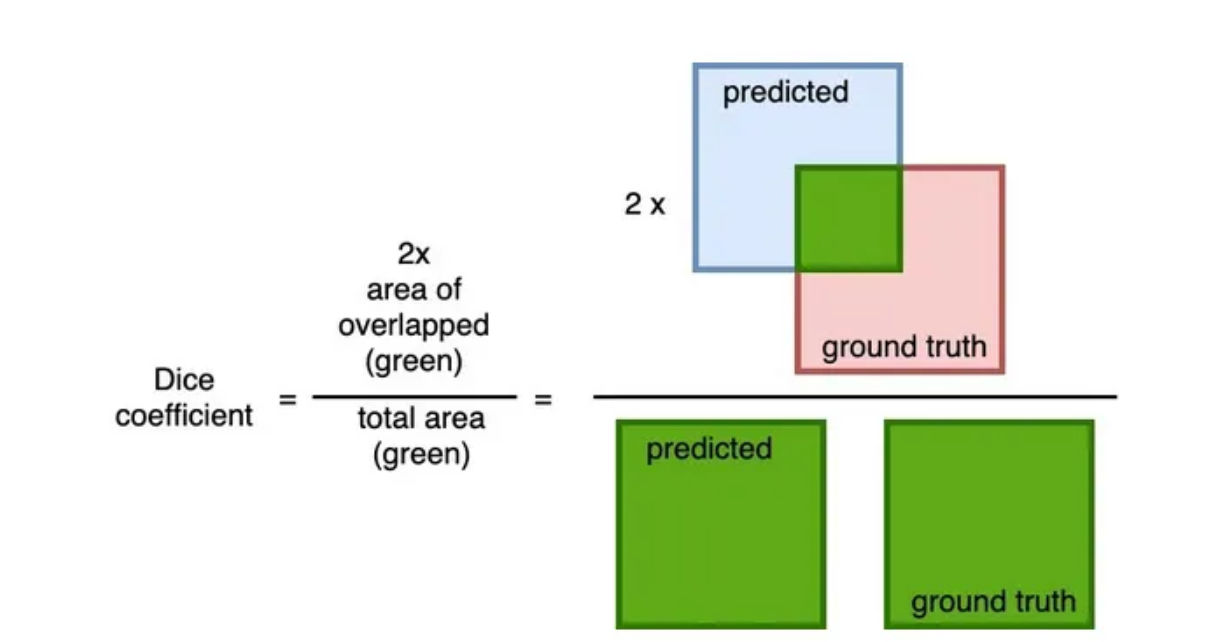
\includegraphics[width=0.7\textwidth]{figures/dice_loss_illustration.png}
    \caption{Visual explanation of the Dice coefficient calculation. The Dice coefficient is computed as the ratio of twice the area of overlap (green) to the total area of both the predicted segmentation and ground truth. Image adapted from \cite{nevilledice2023}.}
    \label{fig:dice_illustration}
\end{figure}

The Dice loss is derived from the Dice coefficient (also known as F1 score), which measures the overlap between the predicted segmentation and the ground truth. The Dice coefficient is defined as:

\begin{equation}
\text{Dice} = \frac{2 |X \cap Y|}{|X| + |Y|}
\end{equation}

where $X$ is the predicted set and $Y$ is the ground truth set. 

